\chapter{Architecture}
\label{chapter:architecture}

The MECOIS setup consists of 3 separate systems, that communicate via \ac{HTTP} (see Figure \ref{fig:basic_system_architecture}). The systems are separated to protect sensitive information.

\begin{figure}[ht]
	
\includegraphics[width=\textwidth]{resources/architecture.png}
	\caption{Basic System Architecture} 
	\label{fig:basic_system_architecture}
\end{figure}

\section{Main System}
\label{sec:main_system}

The main system serves as the central orchestration hub of the MECOIS framework, encompassing all operational responsibilities except for identity management. It is structured as a modular environment composed of several specialized components that facilitate the end-to-end processing of software development metadata, starting from initial data ingestion to the generation of final productivity metrics. 

\subsection{Components}
\label{subsec:components}

Figure \ref{fig:MecoIS_GitHub_Structure} displays an overview of all components. \autocite{github_mecois}

\begin{figure}[ht]
	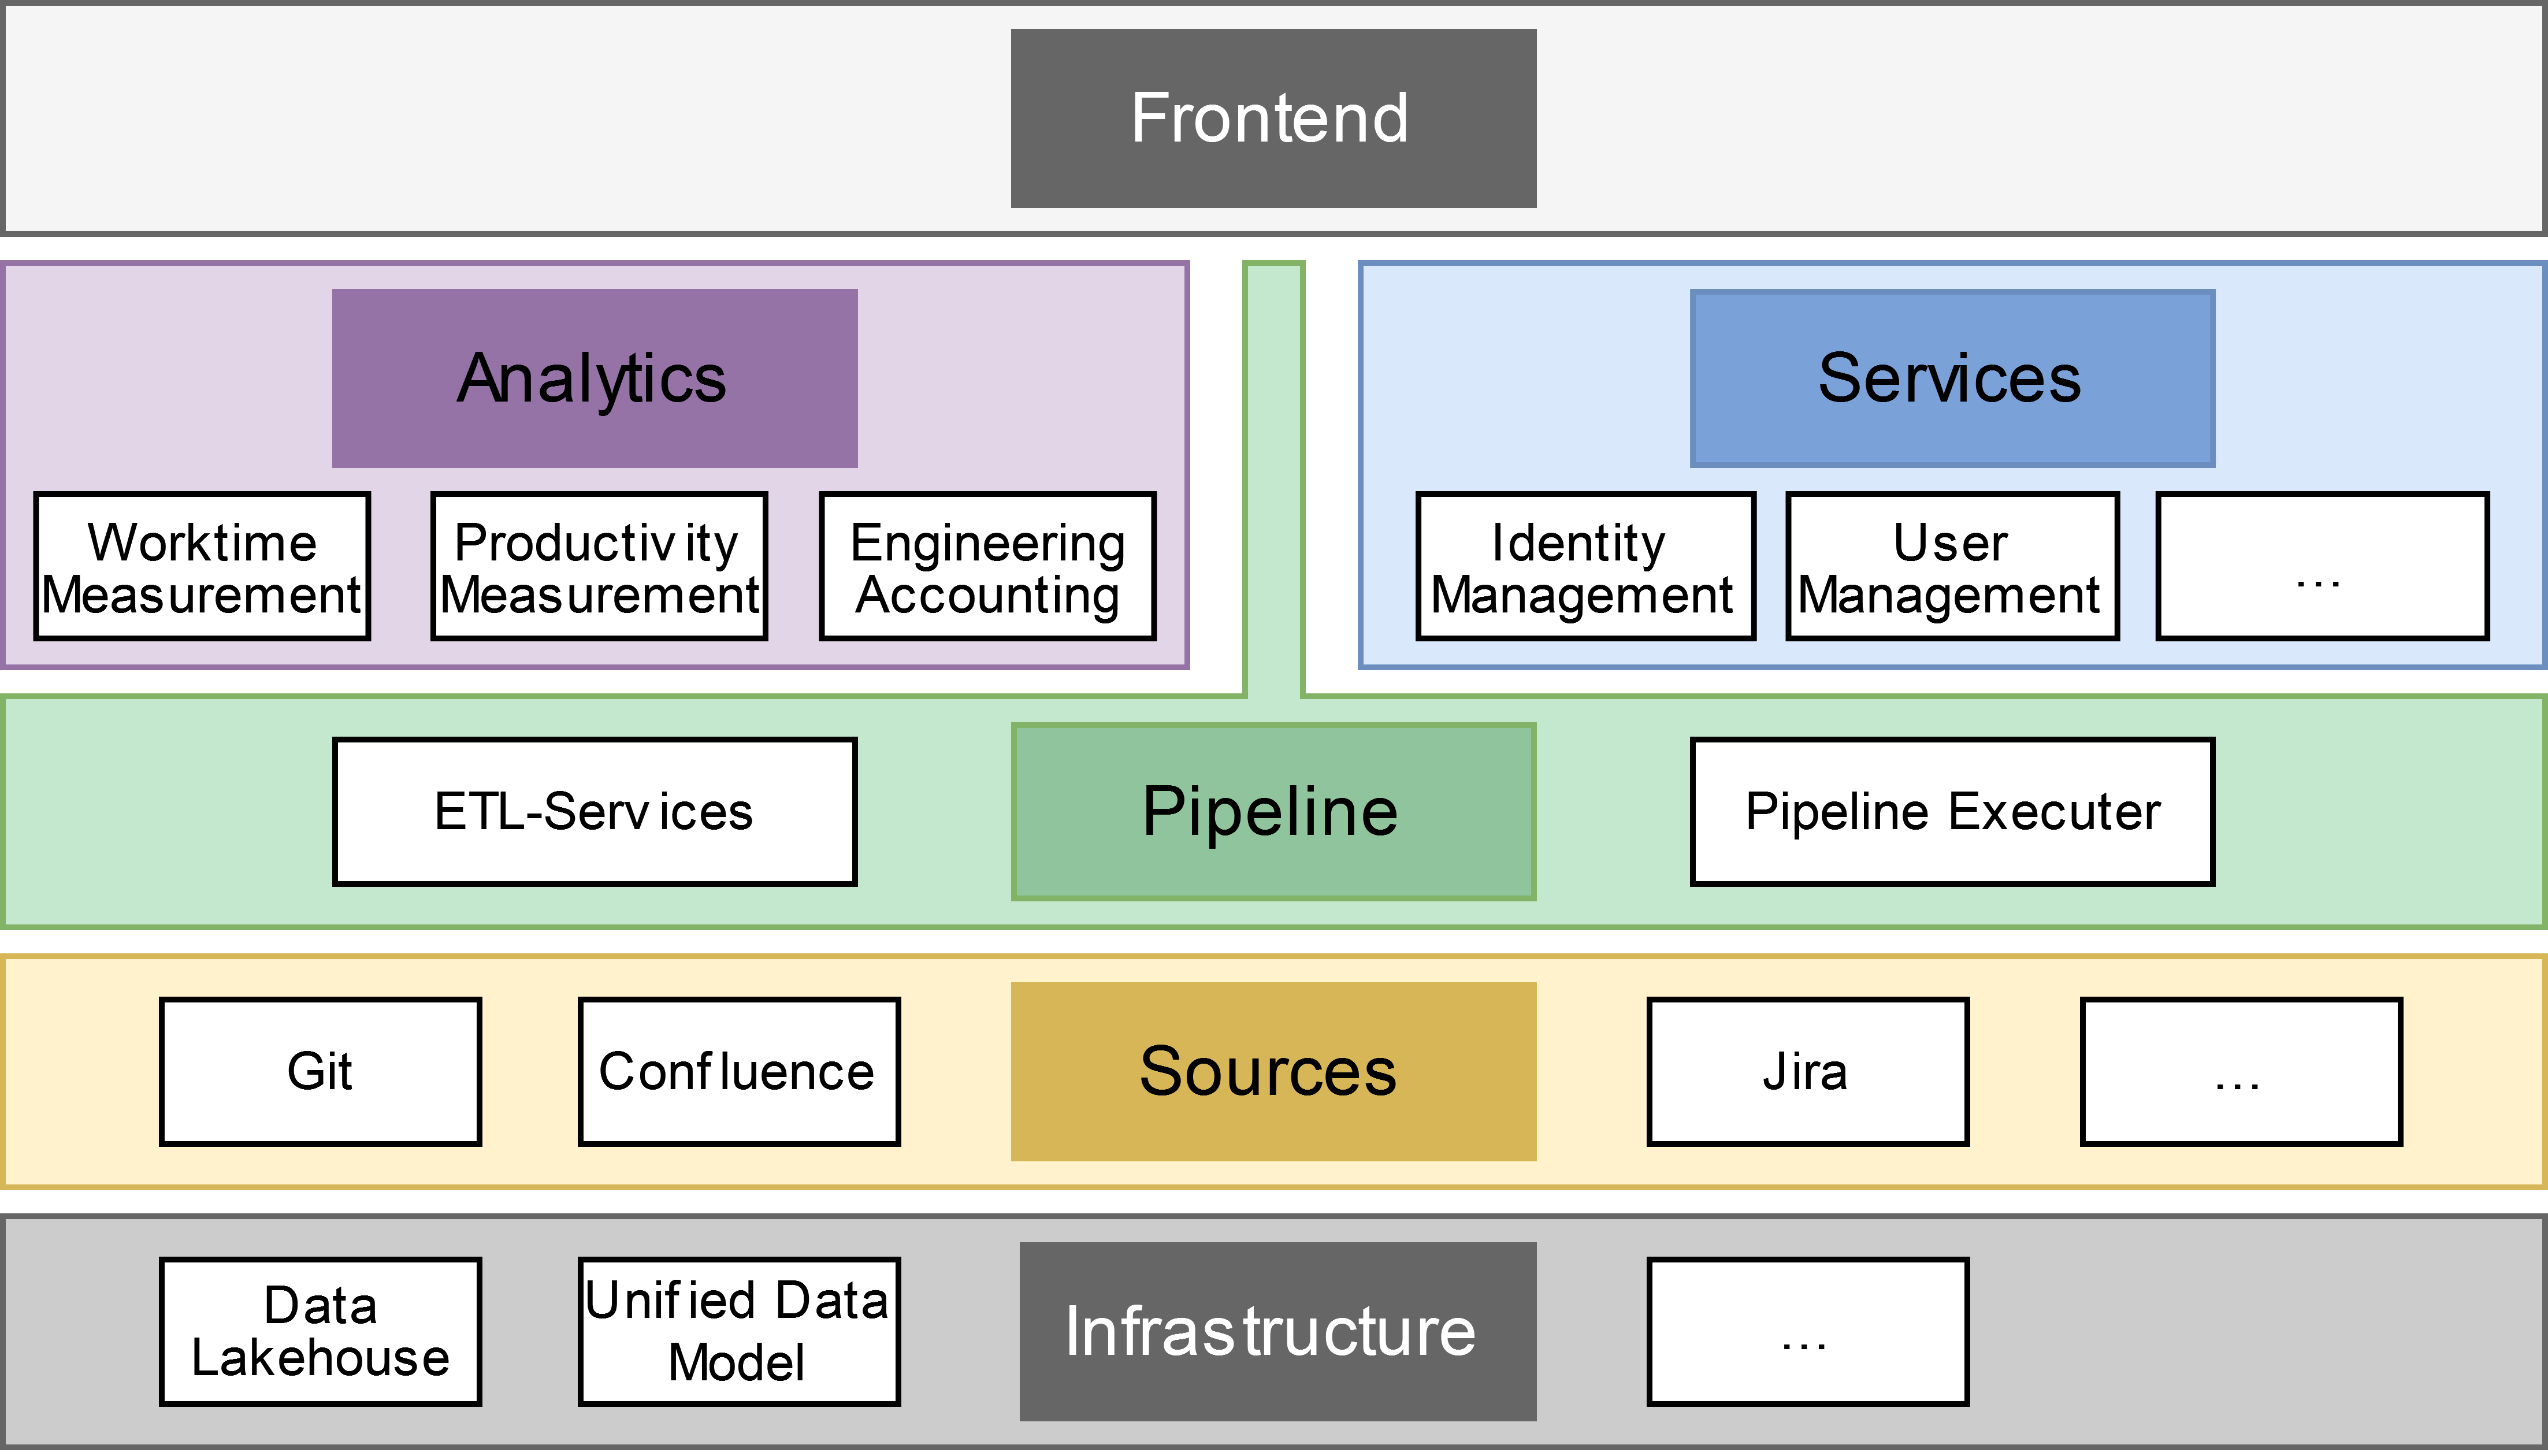
\includegraphics[width=\textwidth]{resources/MecoIS_GitHub_Structure.png}
	\caption{Main System Components \autocite{github_mecois}} 
	\label{fig:MecoIS_GitHub_Structure}
\end{figure}


\subsubsection{Sources}
\label{subsubsec:sources}
The Source component serves as the primary gateway for data ingestion, defining the specific origins of the metadata processed by the MECOIS framework. Currently, the system supports a variety of platforms, including version control systems like Git (interfaced through GitHub and GitLab), documentation tools such as Confluence, and issue trackers like Jira. This architectural layer is designed to be extensible, allowing for the integration of additional data sources in the future. For instance, when querying GitHub, the system retrieves diverse activity-based artifacts, including commits, issue logs, and pipeline execution data.

\subsubsection{Infrastructure}
\label{subsubsec:infrastructure}

The infrastructure layer provides the central data repository for the MECOIS framework, utilizing a data lakehouse architecture to manage complex metadata. A data lakehouse is a unified data architecture that combines the strengths of traditional data lakes and data warehouses, offering a high-performance and governance-friendly environment for storing raw data in diverse formats. It allows organizations to store structured, semi-structured, and unstructured data in a central location where it remains accessible for analytics, machine learning, and reporting without the need for extensive data movement. Within the MECOIS system, information progresses through four sequential stages: raw, bronze, silver, and gold.
\autocite{aws_datalakehouse_2026}

\subsubsection{Pipeline}
\label{subsubsec:pipeline}

The pipelines serve as the operational backbone of the MECOIS framework, responsible for the systematic transformation of development metadata through the various stages of the data lakehouse. Within this architecture, metadata is processed multiple times to evolve from its original, raw state into high-quality, privacy-preserving metrics. This progression is categorized into four distinct states: raw, bronze, silver, and gold. Each pipeline follows a standardized three-step execution model: first, the data is read from the data lake; second, the specific transformations are applied; and third, the results are written back to the repository.


\subsubsection{Analytics}
\label{subsubsec:analytics}
The final phase of the MECOIS framework involves the derivation of high-level metrics from the refined and anonymized data stored within the Silver layer. This stage, characterized as the Silver-to-Gold transformation, generates the structured analytics required for management reporting, productivity assessment, and financial documentation. By applying specialized algorithms to the processed metadata, the system transforms technical artifacts into actionable business insights that allow organizations to quantify the impact of internal collaborative efforts.
Current examples of these analytical applications focus heavily on the economic and temporal quantification of developer contributions:
\begin{itemize}
	 \item \textbf{Cost Calculation in Inner Source:} As explored by \textcite{analytic_cost}, the framework can be utilized to calculate transfer prices and labor costs for Inner Source collaboration by estimating the time worked on individual commits, thereby facilitating fair cost allocation across different organizational units.
	  \item \textbf{Contribution Time Estimation:} Building upon the previous methodology, \textcite{analytic_contribution} provides an improved approach for estimating software contribution time from Git and GitHub metadata. This work addresses real-world implementation challenges such as the disassembly of squashed commits, time zone normalization, and the elimination of statistical outliers to provide a more robust evidential basis for cost calculation.
\end{itemize}


\subsubsection{Services}
\label{subsubsec:services}

Services are helper modules for pipelines and analytics. Such helper modules are:

\begin{itemize}
	\item AI: a framework for communicating with a \ac{LLM}.
	\item config handling: Parses configuration files for pipelines.
\end{itemize}

\subsubsection{Front end}
\label{subsubsec:front_end}

The front end provides a Dashboard for the user-facing components of MECOIS. Figure \ref{fig:mecois_frontend_explorer} shows the Data Explorer tool, where users can examine the data in the data lake. Figure \ref{fig:mecois_frontend_extractor} presents the Data Extractor tool, that can be used to query data from the sources and feed it to the pipelines.

\begin{figure}[ht]
	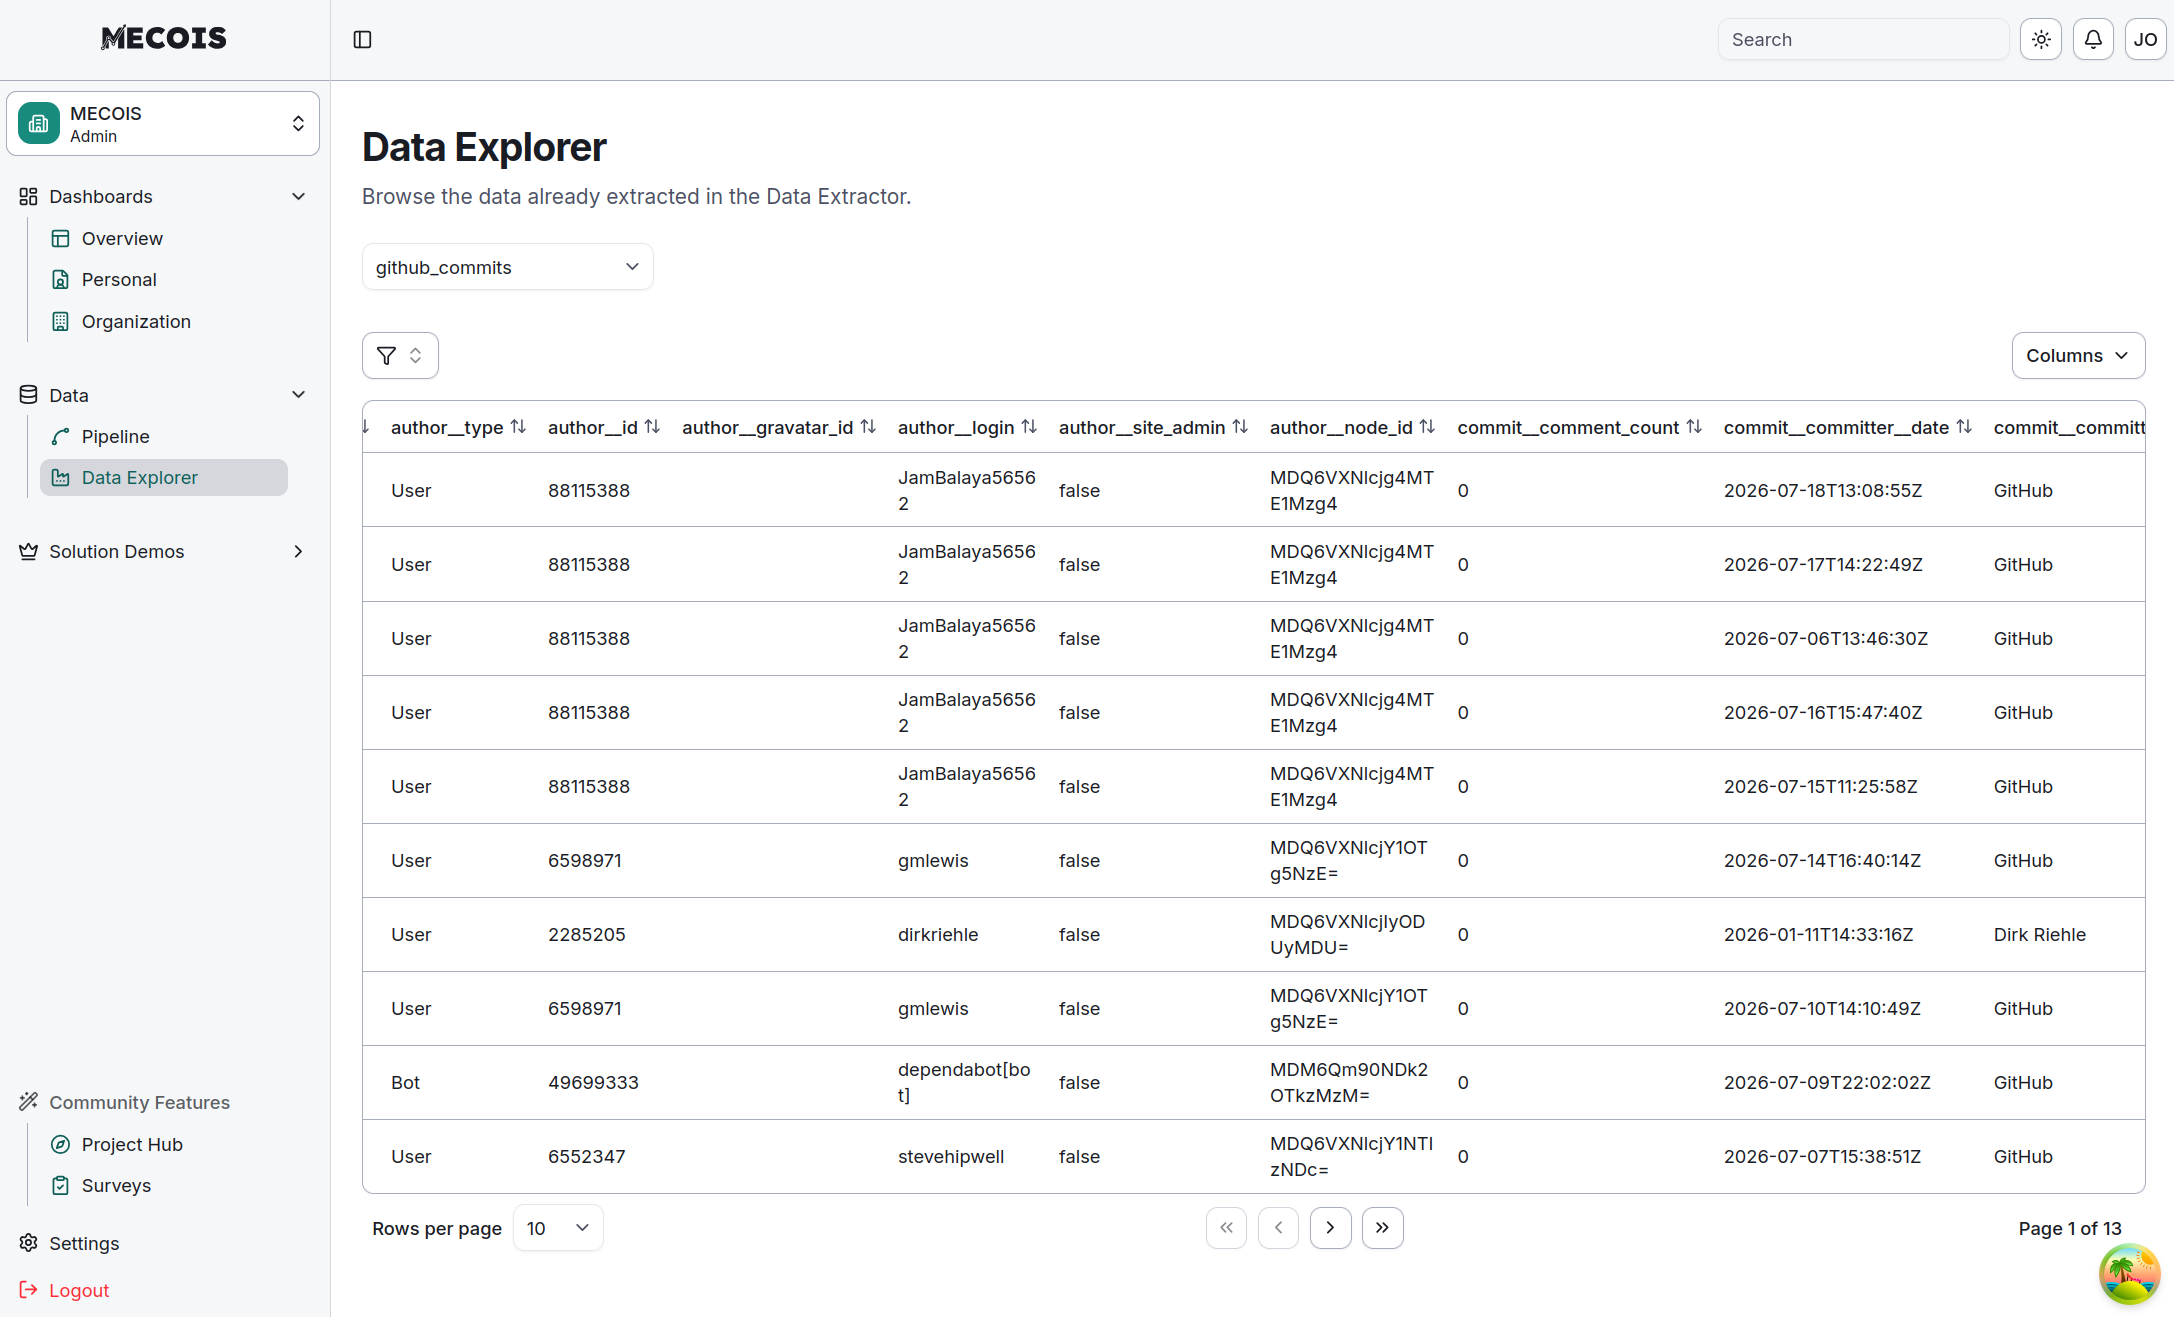
\includegraphics[width=\textwidth]{resources/mecois_frontend_explorer.png}
	\caption{MECOIS Frontend Data Explorer} 
	\label{fig:mecois_frontend_explorer}
\end{figure}

\begin{figure}[ht]
	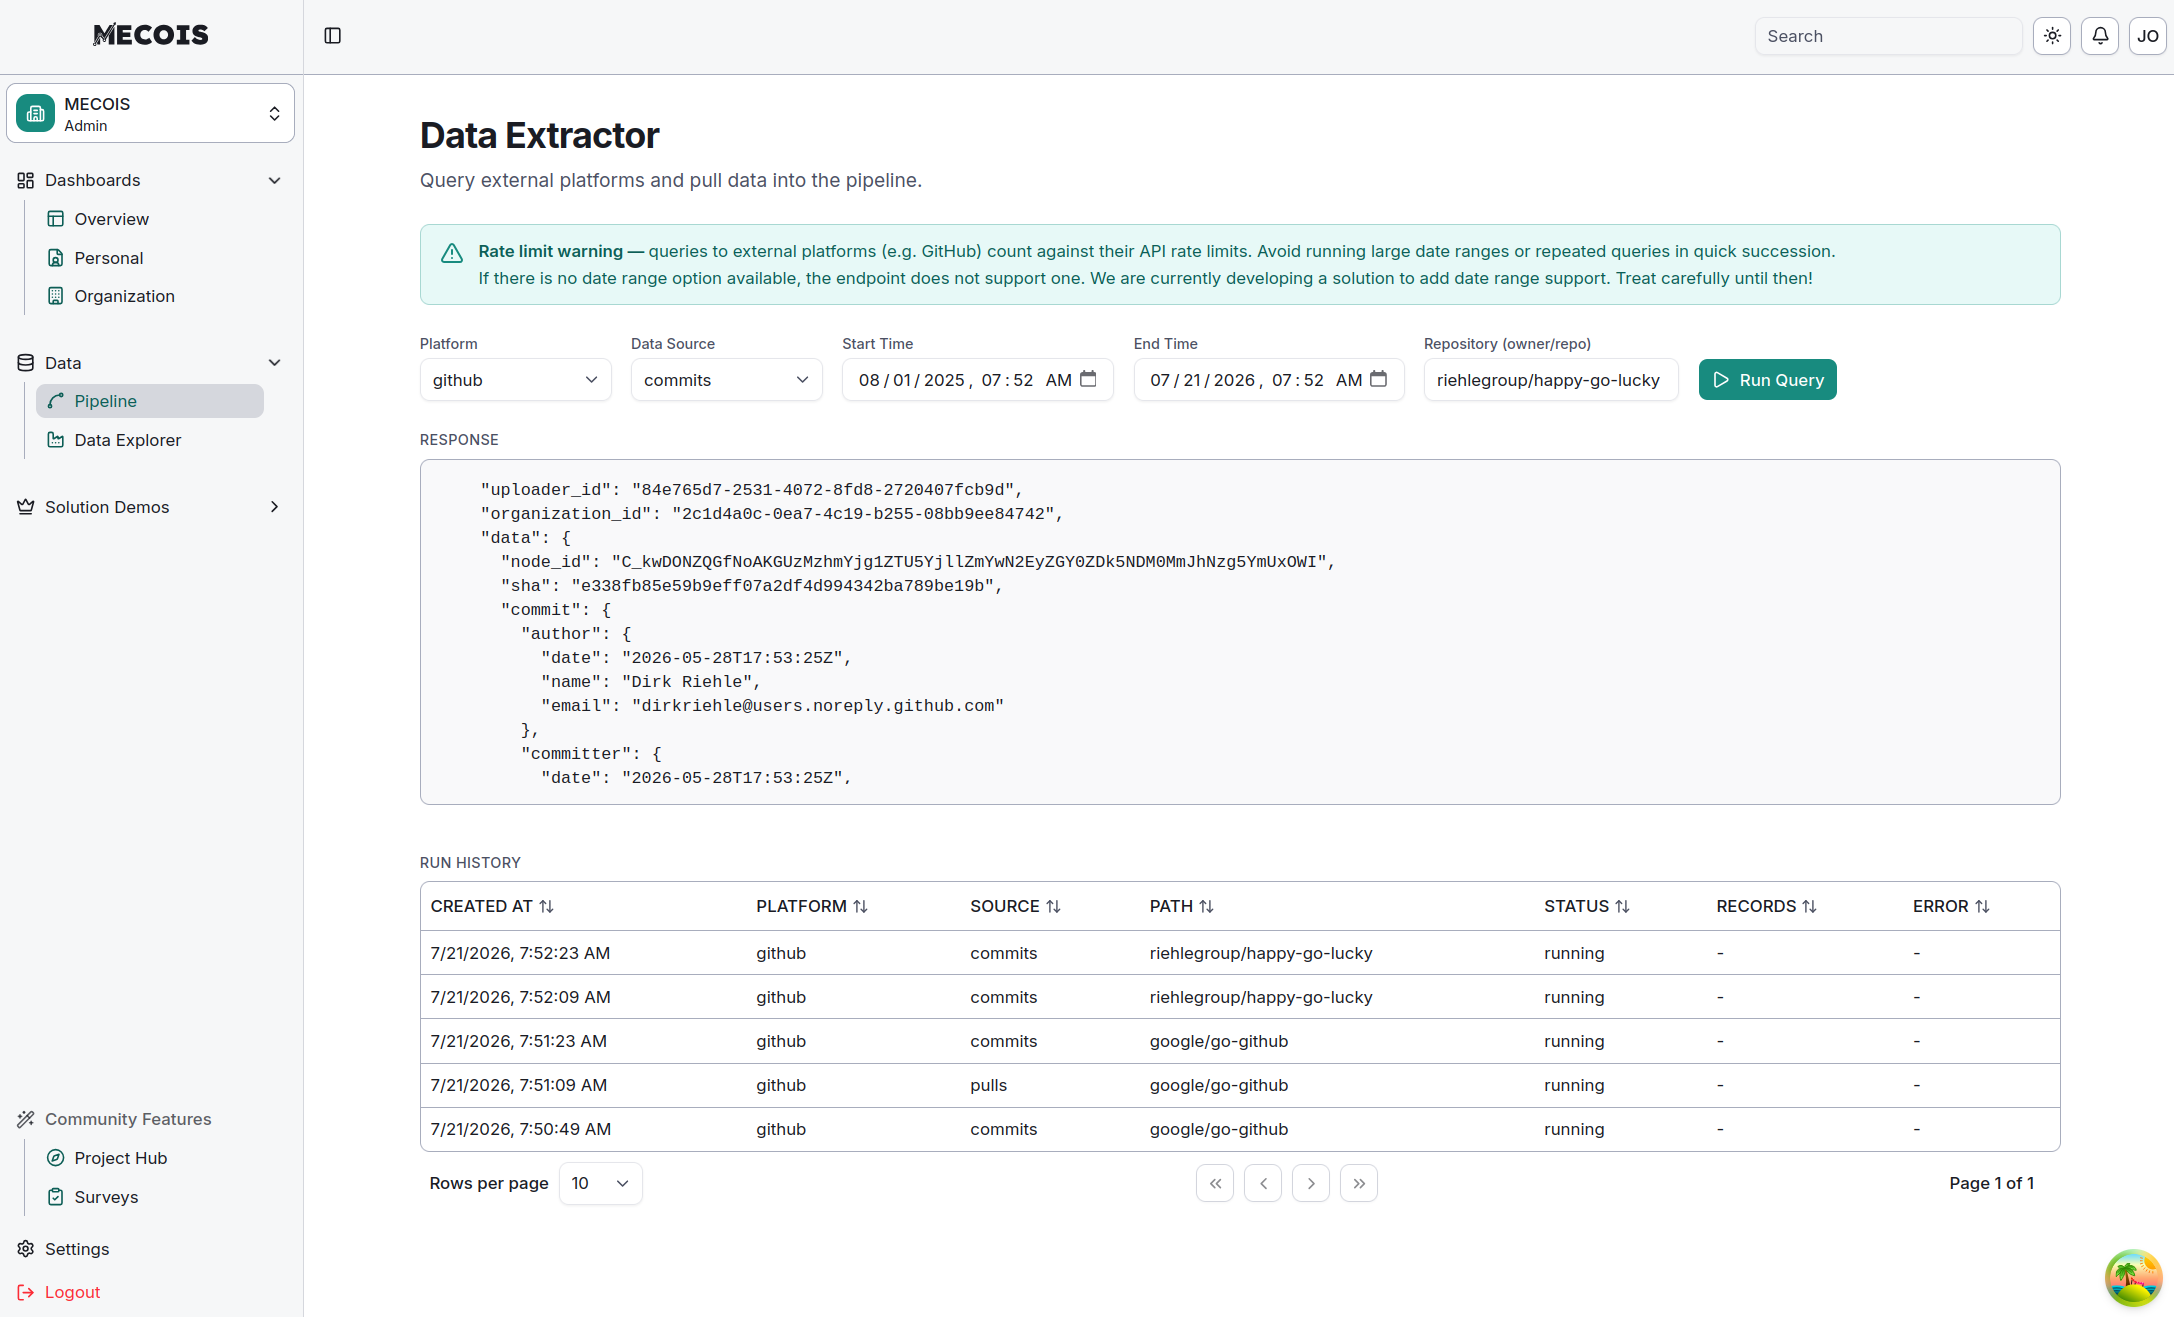
\includegraphics[width=\textwidth]{resources/mecois_frontend_extractor.png}
	\caption{MECOIS Frontend Data Extractor} 
	\label{fig:mecois_frontend_extractor}
\end{figure}

\subsubsection{Orchestrators}
\label{subsubsec:orchestrators}

The orchestrators can be used to run the pipeline. They set up the configuration and run the pipeline for the selected sources.

\subsection{Data Flow}
\label{subsec:dataflow}

Upon successful extraction from the primary sources, the raw metadata is persisted within the data lakehouse in its original \ac{JSON} format to ensure data provenance. This data subsequently undergoes a multi-stage refinement process, systematically evolving through a series of qualitative states defined as bronze, silver, and gold. These transitions are orchestrated by specialized pipelines, each of which adheres to a standardized three-step execution model:
\begin{enumerate}
	\item \textbf{Data Retrieval:} The pipeline initiates by reading the required dataset from the relevant storage tier within the data lake.
	\item \textbf{Transformation:} Specific analytical logic, data cleaning, or privacy-preserving transformations are applied to the records in memory.
	\item \textbf{Data Persistence:} The resulting transformed and enriched records are written back to the subsequent tier of the data lake repository.
\end{enumerate}
A comprehensive overview of these processing stages and the interaction between the various framework components is illustrated in Figure \ref{fig:dataflow}. \autocite{github_mecois}

\begin{figure}[ht]
	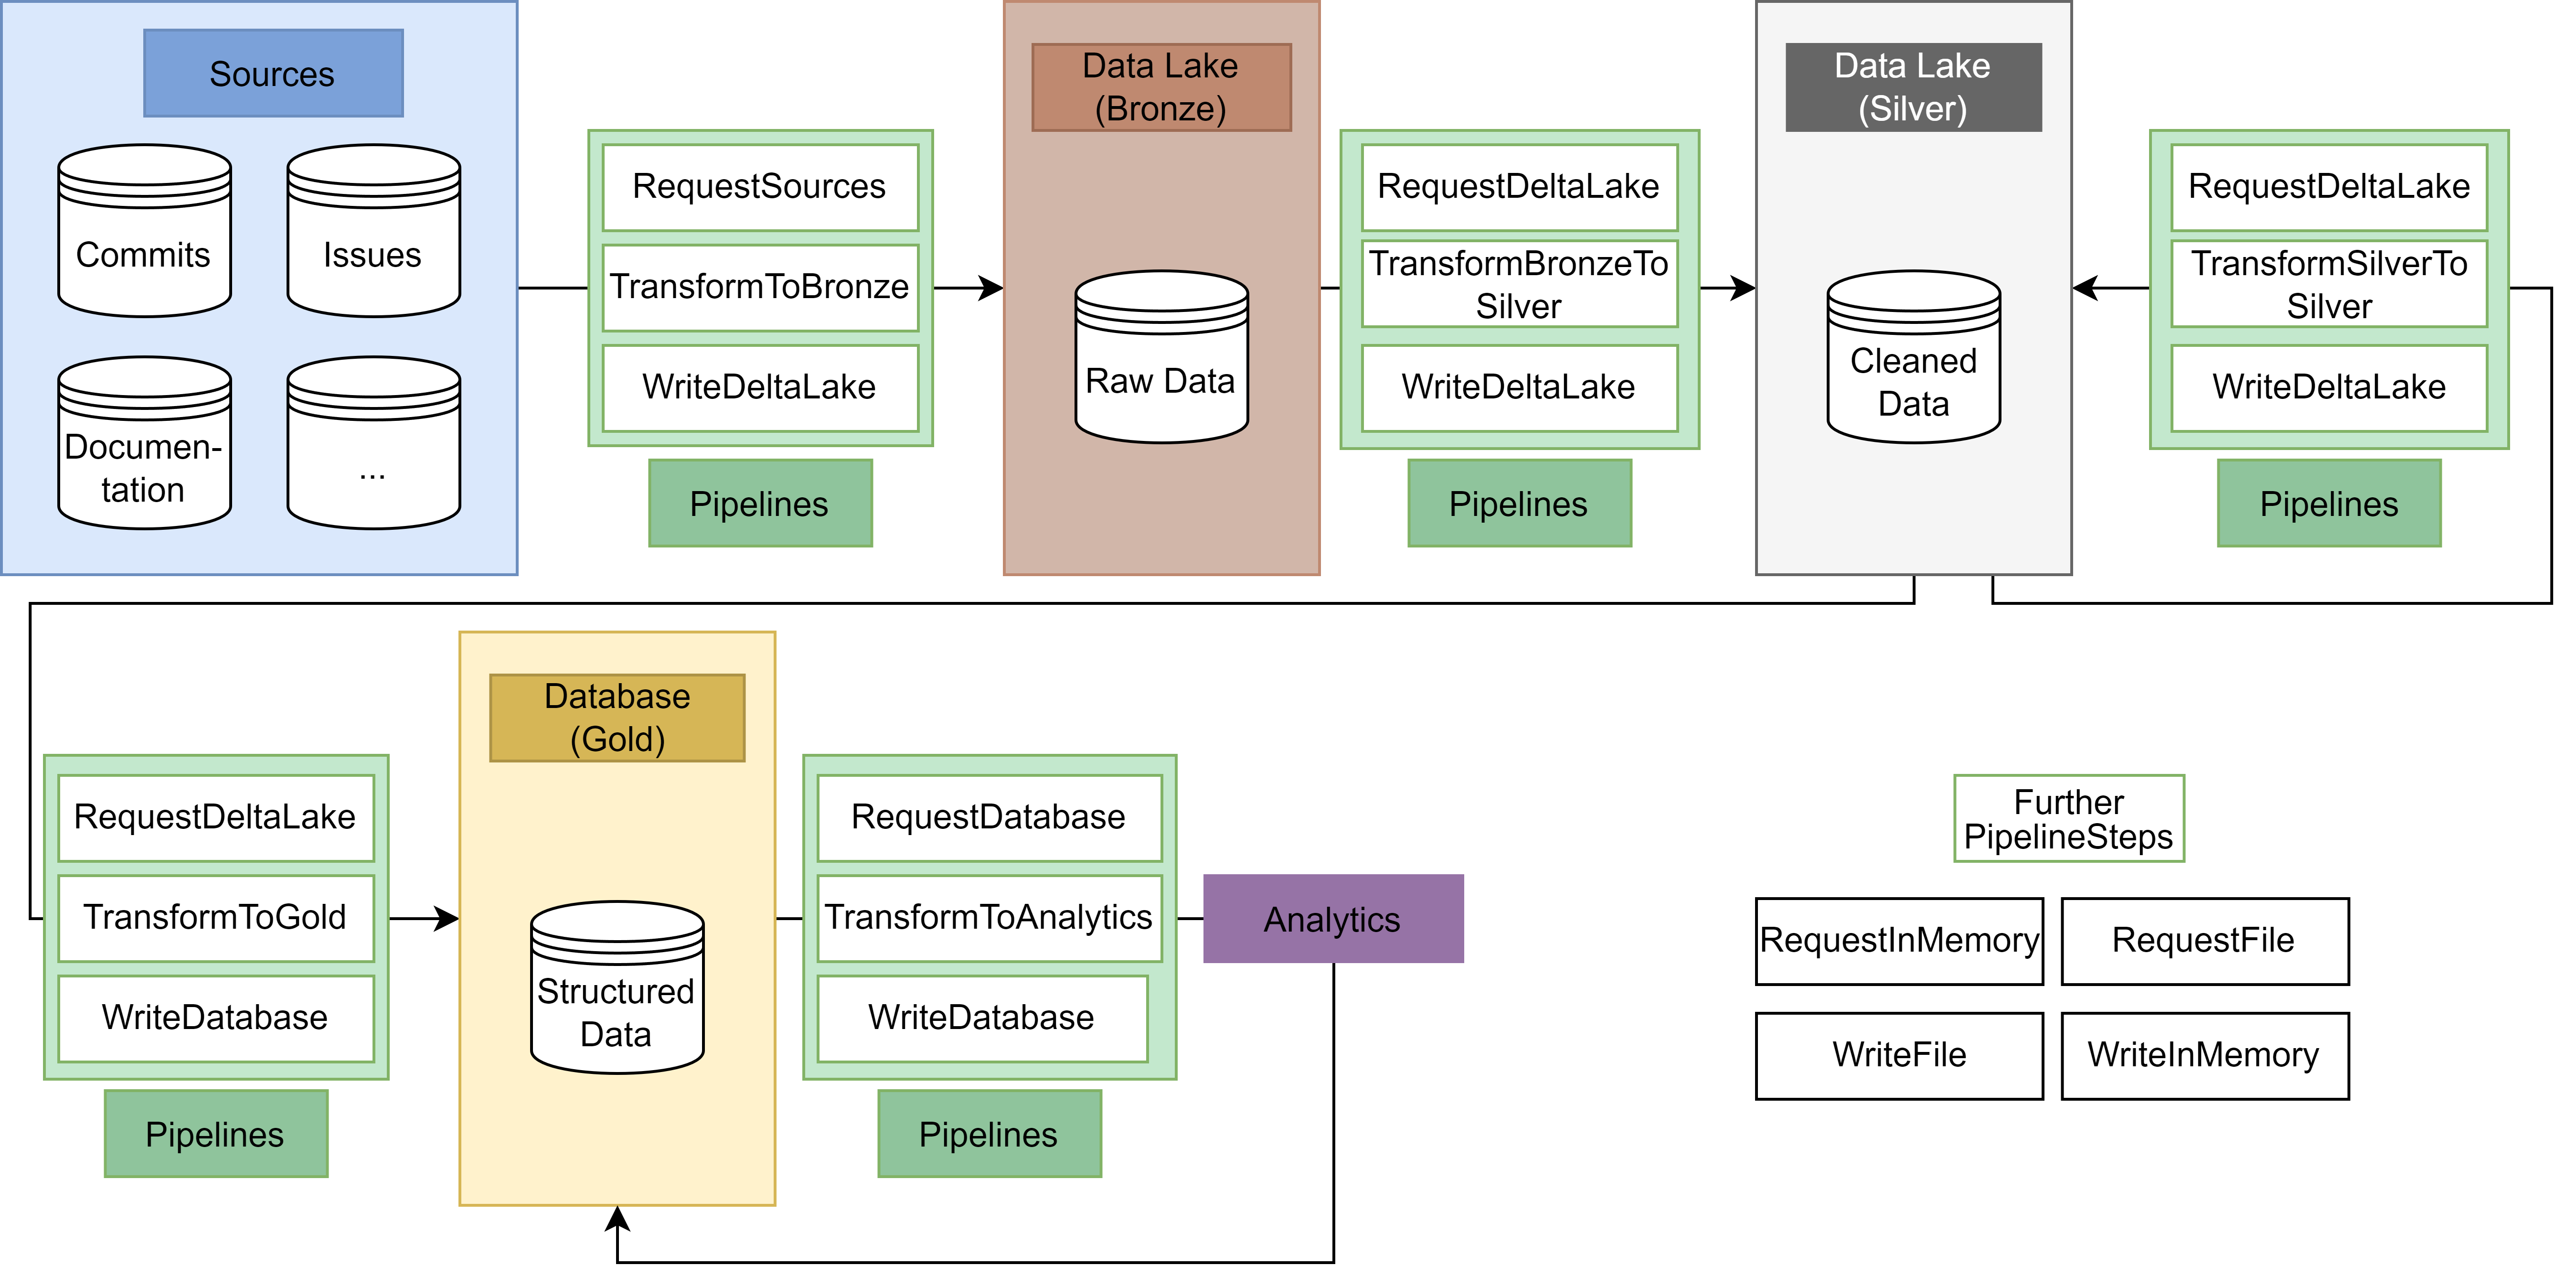
\includegraphics[width=\textwidth]{resources/MecoIS_Pipeline_Structure_Simple.png}
	\caption{Data flow \autocite{github_mecois}} 
	\label{fig:dataflow}
\end{figure}

\subsubsection{JSON to Bronze}
\label{subsubsec:json2bronze}

The \texttt{JSONtoBronzePipeline} processes the raw \ac{JSON} data provided by the sources and writes it unchanged to the Data lake. The data itself is not changed in any way. Each source has an own table.

\subsubsection{Bronze to Silver} \label{subsubsec:bronze2silver}
The \texttt{BronzetoSilverPipeline} serves as the primary refinement stage within the MECOIS framework, transforming raw, ingestion-tier data into a structured and privacy-compliant format suitable for high-level analytics. This pipeline executes a series of sequential transformations designed to enhance data quality, normalize schemas, and ensure adherence to legal privacy standards.

\paragraph{Flatten Table}
Because the bronze storage tier preserves the original nested structure of \ac{JSON} artifacts, the data often contains hierarchical objects that are incompatible with flat relational analytics. For example, a GitHub commit object may contain nested properties for the author, which cannot be natively represented in the simplified bronze schema. To resolve this, the pipeline deconstructs these nested columns into individual, flattened columns, ensuring that each field contains only a single data point for subsequent statistical evaluation.

\paragraph{Drop Irrelevant Columns}
To optimize storage efficiency and focus on relevant metrics, the pipeline identifies and removes attributes that offer no analytical value to the productivity index. Metadata such as the URL for a GitHub user's avatar is discarded, which reduces the dimensionality of the dataset and ensures that only pertinent information is persisted in the silver tier.

\paragraph{Fix Dates} Temporal metadata extracted from development sources is initially stored as unformatted strings during the bronze stage. This transformation step casts these strings into native timestamp objects, allowing the database to store them natively and facilitate efficient time-series analysis. By normalizing these attributes, the framework ensures temporal consistency and computational accuracy across all derived datasets.

\paragraph{Anonymize Data}
A central function of this pipeline is the integration of privacy-preserving measures through the decoupled anonymization service. During this phase, the data is transmitted to the service via the \texttt{change\_identities} endpoint. This process ensures that the resulting silver-tier data meets the privacy requirements while remaining analytically useful.

\paragraph{Add UUID}
The pipeline generates a deterministic \ac{UUID} for each record by concatenating specific columns and hashing the result.

\subsubsection{Silver to Silver}
\label{subsubsec:silver2silver}

The Silver-to-Silver processing tier is responsible for maintaining the synchronization and accuracy of the data lakehouse as contributor information evolves within the identity management system. Since the SortingHat system frequently undergoes updates—such as the merging of fragmented developer profiles or changes in organizational affiliations—the silver-tier datasets must be adjusted to reflect these new identities. To address this, the \texttt{UpdateIdentityPipeline} monitors modifications within SortingHat and triggers a re-evaluation of previously processed records in the data lake. By invoking the \texttt{update\_identities} endpoint of the anonymization service, the pipeline ensures that all pseudonymized identifiers and organizational mappings remain consistent with the latest identity data, thereby preserving the reliability of the longitudinal metrics derived by the MECOIS framework.

\subsubsection{Silver to Gold}
\label{subsubsec:silver2gold}

The transition from the silver to the gold tier does not rely on a singular, monolithic pipeline. Instead, the various analytical modules themselves function as the silver-to-gold pipelines, as each specific analytic consumes the cleaned and anonymized silver data to derive specialized metrics. This stage represents the final transformation where refined metadata is converted into high-level, structured insights for the MECOIS Productivity Index.

\subsubsection{Gold to Gold}
\label{subsubsec:gold2gold}

Certain analytical applications may require a specialized mechanism to refine or update previously generated metrics. This iterative processing stage is defined as a gold-to-gold transformation, ensuring that the stored metrics can be adjusted or maintained over time without necessitating a full re-processing of the underlying silver-tier data.

\section{Anonymization System}
\label{sec:anonymization_system}

The anonymization system provides the anonymization service, that anonymizes the data according to the \ac{GDPR} and \ac{BDSG}.
It provides a client library for sending data and requesting identities. 

\section{Identity Management System}
\label{sec:identity_management_system}

The identity management system serves as the primary repository for all individual-related data within the MECOIS framework. For this purpose, the project integrates SortingHat, a specialized component of the GrimoireLab toolset developed by CHAOSS. This software is distributed under the GPL-3.0 license. To address the frequent fragmentation of identities across different platforms such as Git, Slack, and Jira, SortingHat provides a robust infrastructure for unifying disparate usernames and aliases into cohesive individual profiles. This unification process allows the system to aggregate multiple accounts belonging to a single person into a centralized entity. Furthermore, these consolidated individuals can be organized into hierarchical structures, ranging from specific teams to broader organizational units.

\subsection{Identities}

\begin{figure}[ht] \centering 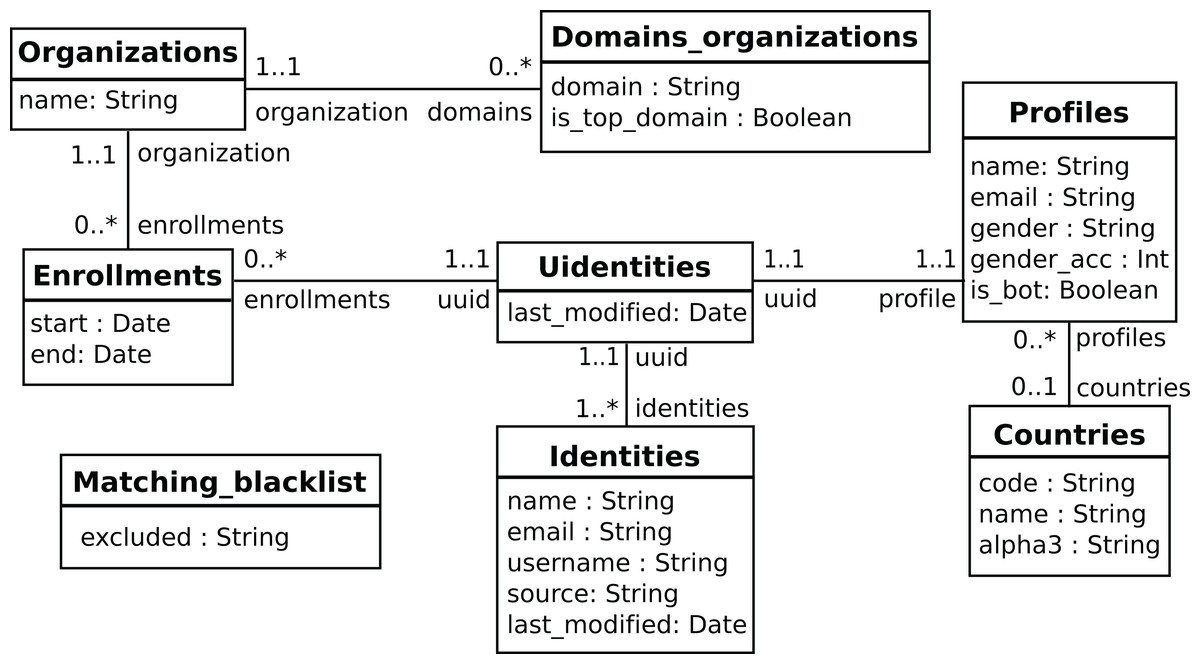
\includegraphics[width=\textwidth]{resources/SortingHatUML.jpg} \caption{SortingHat UML diagram \autocite{duenas2021grimoirelab}} \label{fig:sortinghat_uml_diagram} \end{figure}

The conceptual mapping of identities within SortingHat is illustrated in the UML diagram shown in Figure \ref{fig:sortinghat_uml_diagram}. This architecture enables the system to pool diverse identities—such as various GitHub accounts or email addresses—into a single individual representation. Each unique individual is assigned a deterministic \ac{UUID}, which serves as a stable identifier linked to a profile containing relevant personal information. Beyond simple identification, the system facilitates the association of these individuals with specific organizations, supporting the longitudinal tracking of developer trajectories and cross-platform activity metrics.

\subsection{Front end Dashboard}
\label{subsubsec:front_end_dashboard}


SortingHat incorporates a dedicated web-based dashboard designed to facilitate manual identity curation and the management of contributor affiliations. This interface allows researchers and administrators to oversee and refine the unification of digital profiles, complementing the system's automated merging algorithms. \autocite{sortinghat_interface}
The dashboard is organized into three primary functional modules:
\begin{itemize}
	\item \textbf{Workspace:} This area serves as a staging environment for tracking specific individual profiles that require pending administrative actions, providing a focused workflow for identity resolution.  \autocite{sortinghat_interface}
	\item \textbf{Individuals:} This module contains a centralized registry of unique profiles. Within the SortingHat framework, a profile represents a single human contributor, while identities correspond to their various accounts across disparate platforms, such as Git, GitHub, Slack, or mailing lists. This section allows for the aggregation of multiple digital aliases and email addresses into a cohesive individual representation. \autocite{sortinghat_profiles} \autocite{sortinghat_interface}
	\item \textbf{Organisation:} This section manages the list of affiliations where individuals are employed or enrolled, enabling the association of contributors with their respective organizational units. \autocite{sortinghat_interface}
\end{itemize}
A Screenshot of the front-end environment is provided in Figure \ref{fig:sortinghat_frontend}. To comply with data privacy standards, personal identifiers within this screenshot have been redacted. An official uncensored version of the individuals board is illustrated in Figure \ref{fig:sortinghat_frontend_individuals}.

\begin{figure}[ht]
	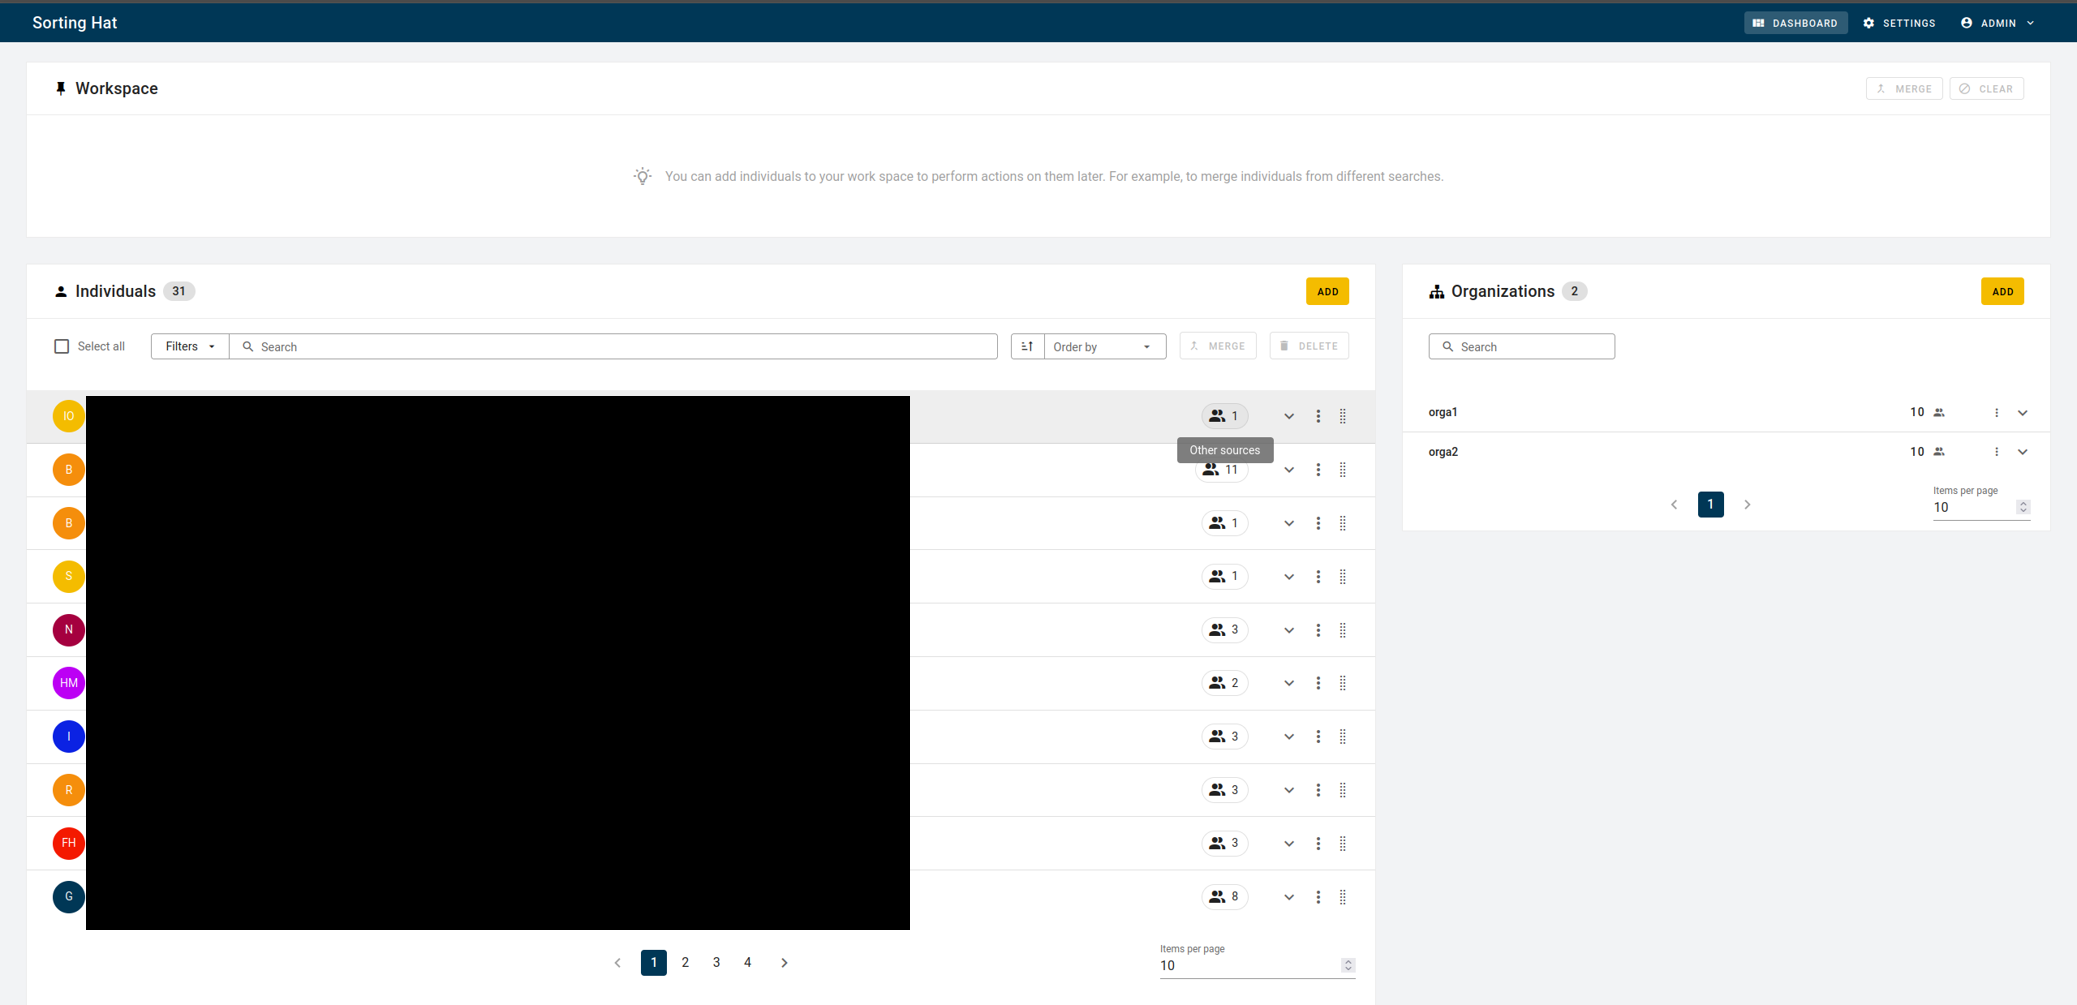
\includegraphics[width=\textwidth]{resources/sortinghat_dashboard.png}
	\caption{SortingHat front end (individuals are censored for privacy reasons)} 
	\label{fig:sortinghat_frontend}
\end{figure}

\begin{figure}[ht]
	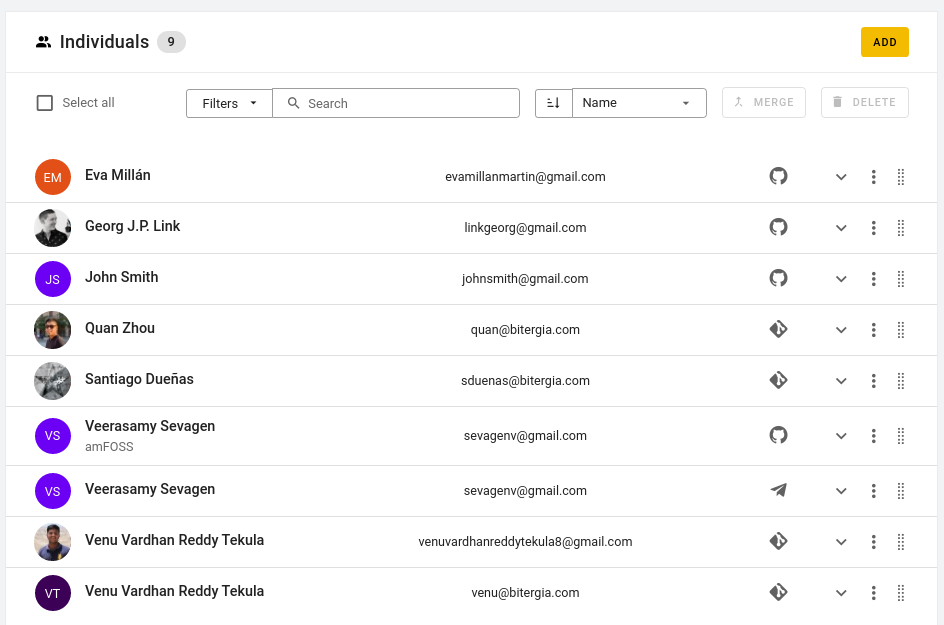
\includegraphics[width=\textwidth]{resources/sortinghat_individuals.png}
	\caption{SortingHat individuals section (uncensored) \autocite{sortinghat_interface}} 
	\label{fig:sortinghat_frontend_individuals}
\end{figure}

\subsection{API}
\label{subsubsec:api}

The SortingHat also provides an \ac{API} for automating interactions, like listing, updating and deleting individuals.
